\documentclass[11pt]{article}
\usepackage[margin=1in]{geometry}
\usepackage{amsmath,amssymb}
\usepackage{enumitem}
\usepackage{booktabs}
\usepackage{graphicx}

\DeclareMathOperator{\bias}{bias}

\pagestyle{plain}

\begin{document}

\begin{center}
{\Large \textbf{Statistics 256: Causality}} \\[6pt]
{\large In-class Activity 7: Sensitivity --- Use, Interpretation, and Abuses}
\end{center}

\vspace{4pt}
\noindent\textbf{Name(s):} \hrulefill

\vspace{12pt}

\noindent\textbf{Setup.}  A study estimates the effect of a binary treatment on an outcome, adjusting for covariates $\mathbf{X}$.  The augmented regression table:

\medskip
\begin{center}
\begin{tabular}{lrrrrrr}
\toprule
Treatment & Est. & SE & $t$ & $R^2_{Y\sim D|\mathbf{X}}$ & RV & $\mathrm{RV}_{\alpha=0.05}$ \\
\midrule
\textit{Treatment} & 0.30 & 0.10 & 3.00 & 1.5\% & 11.4\% & 4.0\% \\
\bottomrule
\end{tabular}
\end{center}
\medskip
\noindent $\mathrm{df} = 600$.  The strongest observed covariate is $X_1$, with $R^2_{Y\sim X_1 \mid \mathbf{X}_{-1},D} = 8\%$ and $R^2_{D \sim X_1 \mid \mathbf{X}_{-1}} = 4\%$.

\vspace{14pt}

%%% Q1
\noindent\textbf{Question 1: Plain English} (answer in one sentence each)
\medskip
\begin{enumerate}[label=(\alph*)]
\item What does $\mathrm{RV} = 11.4\%$ tell us?
\vspace{1.2cm}

\item What does $\mathrm{RV}_{\alpha=0.05} = 4.0\%$ tell us?  Why is it smaller than the RV?
\vspace{1.4cm}

\item What does $R^2_{Y\sim D|\mathbf{X}} = 1.5\%$ tell us?
\vspace{1.2cm}
\end{enumerate}


%%% Q2 (new: FWL)
\noindent\textbf{Question 2: FWL check}.Consider the linear regression of $Y$ on $D$ and $\mathbf{X}$. Using Frisch--Waugh--Lovell, restate the coefficients you get on $D$ as the result of a bivariate regression. 
\vspace{2.5cm}



%%% Q3 (was Q2)
\noindent\textbf{Question 3: Spot the abuse}. What is problematic with this statement: \textit{``The RV is 50\%, that's really high --- we don't need to worry about unobserved confounding.''}
\vspace{1.3cm}

\clearpage

%%% Q4 (was Q3)
\noindent\textbf{Question 4: Read the contour}

\medskip
\noindent For hypothetical $(R^2_{D\sim Z|\mathbf{X}}, R^2_{Y\sim Z|\mathbf{X},D})$, the plots show the adjusted point estimate (left) and adjusted $t$-statistic (right).  Diamond markers indicate confounder strengths $1\times$, $2\times$, $3\times$ that of $X_1$.

\begin{center}
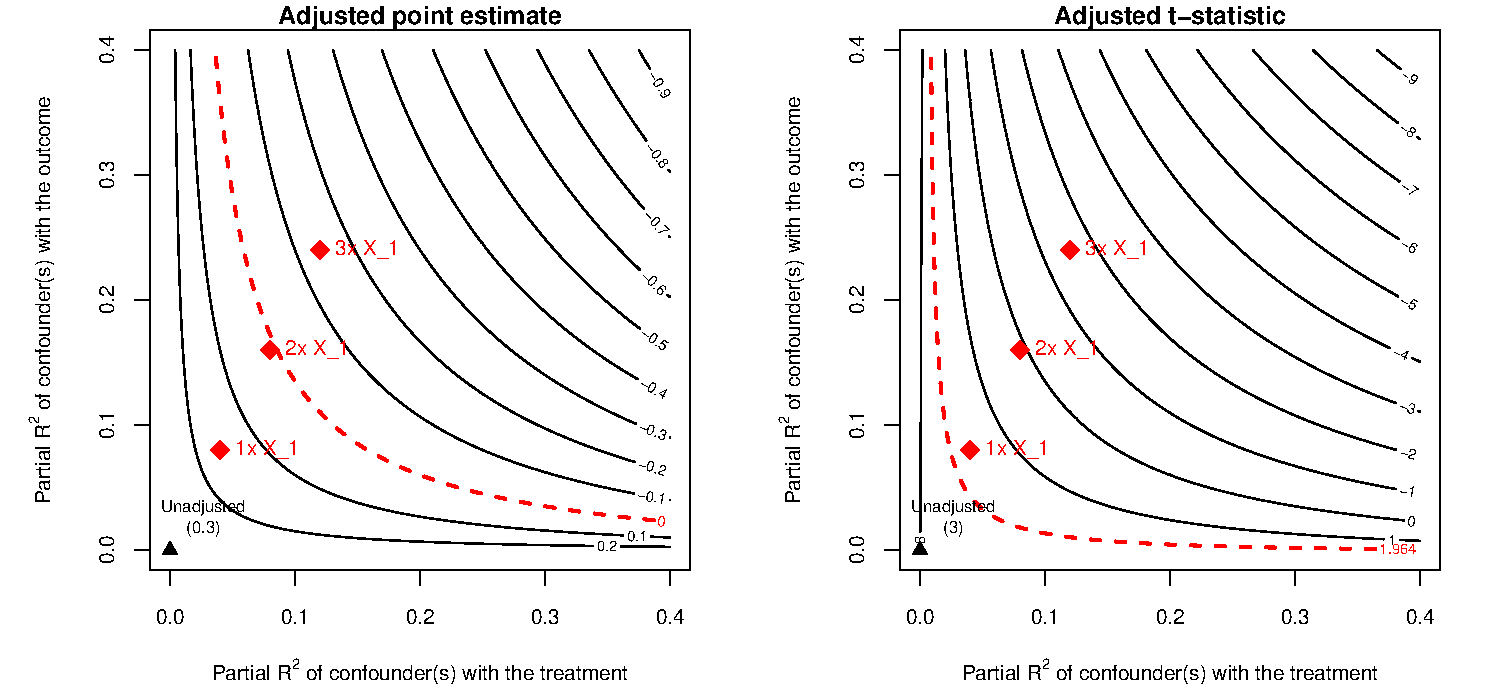
\includegraphics[width=\textwidth]{activity07_contour.pdf}
\end{center}

\medskip
\begin{enumerate}[label=(\alph*)]
\item Would the \textit{point estimate} be driven to zero by a confounder $1\times$ as strong as $X_1$?
\vspace{2.5cm}

\item Is \textit{significance at $\alpha = 0.05$} lost when the confounder is $1\times$ as strong as $X_1$?
\vspace{2.5cm}

\item Roughly how strong (in multiples of $X_1$) would a confounder have to be to drive the \textit{point estimate} to zero?
\vspace{1.5cm}
\end{enumerate}

\end{document}
